%!TEX root = ../../main.tex
\setcounter{section}{2}
\section{Methodology}
\label{sec:methodology}

	The aim of the thesis is to investigate the relation between linguistic typology and cross-lingual transfer. To this end, the methodology involves a typologically-informed, three-stage finetuning setup outlined in Section~\ref{sub:finetuning_setup}. The model~-- described in Section~\ref{sub:model}~-- is finetuned for dependency parsing in a variety of languages, the selection of which is clarified in Section~\ref{sub:language_selection}. Dependency parsing was chosen as a task for a number of reasons. Firstly, the Universal Dependencies (UD)~\cite{nivre-etal-2016-universal} project provides a large number of uniform datasets in many different languages, facilitating cross-lingual comparisons on the same task. Secondly, constructing a correct dependency tree for a sentence in a given language requires knowledge of the syntactic features of that language. Therefore, it is to be expected that dependency parsers encode language-specific syntactic information. In turn, this may mean that typological similarity plays a bigger role in successful cross-lingual transfer than it would with other tasks. How the results obtained from the setup serve to answer the research questions is explained in Section~\ref{sub:experiments}.

	\subsection{Model}
	\label{sub:model}
		The model used was implemented from the ground up, adapting Kondratyuk \& Straka's~\cite{kondratyuk-straka-2019-75} UDify model to better fit the setup of this thesis. In particular, an input token $j$ is encoded using M-BERT~\cite{devlin-etal-2019-bert} to obtain output $U_{i,j}$ at each layer $i \in [1...12]$. A weighted sum $r_j$ is then calculated as follows:

		$$
			r_j = \eta \sum_{i=1}^{12}U_{i,j} \cdot \text{softmax}(w)_i
		$$

		\noindent with $\eta$ a trainable scalar and $w$ a vector of trainable scalar mixing weights. Next, $r_j$ is passed through separate biaffine attention classifiers~\cite{dozat-manning-2016-deep} for predicting the dependency arc and its label. The input to the classifiers comes from four separate MLPs with 256 (arc) or 768 (dep) hidden dimensions and ELU non-linear activation:

		\begin{align*}
			H_{\text{arc-head}, j} &= \text{ELU}(W_{\text{arc-head}}r_j + b_{\text{arc-head}}) \\
			H_{\text{arc-dep}, j} &= \text{ELU}(W_{\text{arc-dep}}r_j + b_{\text{arc-dep}}) \\
			H_{\text{tag-head}, j} &= \text{ELU}(W_{\text{tag-head}}r_j + b_{\text{tag-head}}) \\
			H_{\text{tag-dep}, j} &= \text{ELU}(W_{\text{tag-dep}}r_j + b_{\text{tag-dep}})
		\end{align*}

		\noindent The classifiers then score all possible dependency arcs:

		\begin{align*}
			\mathcal{S}_\text{arc} &= H_{\text{arc-head}, j} \mathbf{W}_{\text{arc}} H_{\text{arc-dep}, j}^{\top} + \mathbf{b}_{\text{arc}} \\
			\mathcal{S}_\text{tag} &= H_{\text{tag-head}, j} \mathbf{W}_{\text{tag}} H_{\text{tag-dep}, j}^{\top} + \mathbf{b}_{\text{tag}}
		\end{align*}

		\noindent Finally, the Chu-Liu/Egmonds algorithm~\cite{chu-1965-shortest} is used to obtain the most probably dependency tree based on $\mathcal{S}_\text{arc}$ and $\mathcal{S}_\text{tag}$. 


	\subsection{Finetuning Setup}
	\label{sub:finetuning_setup}
		As stated, the finetuning setup follows three stages where it first adapts to a source language, then optionally to one of four auxiliary languages, and finally to one of four target languages:

		\begin{list}{}{\leftmargin=\parindent \rightmargin=0.5\parindent}
			\item
			\begin{enumerate}[label=Stage \arabic*:, leftmargin=*, align=left]
			    \item The goal of the first stage is to instill general knowledge of the task at hand. To this end, the model is finetuned on a treebank in the source language, German, resulting in the model \m{deu};
			    \item In the optional second stage, \m{deu} is finetuned on one of the auxiliary languages $\ell \in \{\textit{nld}, \textit{nor}, \textit{ces}, \textit{fin}\}$\footnote{Dutch, Norwegian, Czech, and Finnish.} to obtain four versions of \m{$\ell$};
			    \item \m{deu} and each \m{$\ell$} finetuned on each of the target languages $\lambda \in \{\textit{gsw},$ $\textit{fao},$ $\textit{hsb},$ $\textit{vep}\}$,\footnote{Swiss German, Faroese, Upper Sorbian, and Veps.} resulting in 4 instances of \m{deu,$\lambda$} and 16 instances of \m{$\ell$,$\lambda$}.
			\end{enumerate}
		\end{list}

		In Stage 1, the model is finetuned over the course of 50 epochs on the full German training set with the Adam optimizer~\cite{kingma-ba-2015-adam} and a cosine-based learning rate scheduler with 15\,\% warmup. In Stages 2 \& 3, the training sets are matched in size by randomly sampling a fixed number of examples from each training set. In the second stage, the model is finetuned on 10\,000 examples from each of the auxiliary languages' treebanks over the course of 100 epochs. In the third stage, the model is finetuned on 50 examples from each of the target languages' treebanks over the course of 2 epochs. An overview of the hyperparameters used is given in Appendix~\ref{app:hyperparameters}.\notetoself{This is not currently true}

	\subsection{Language Selection}
	\label{sub:language_selection}
		Broadly speaking, language selection is based on their representation in M-BERT's pre-training data as reported by Wu \& Dredze~\cite{wu-dredze-2020-languages}, as well as their mutual typological similarities. Here, typological similarity is quantified as the cosine similarity between each of the languages' binary \texttt{syntax\_knn} feature vectors from the URIEL knowledge base~\cite{littell-etal-2017-uriel}. Each dimension of those vectors indicates the presence or absence of a syntactic property. An overview of the selected languages and their respective treebanks is shown in Table~\ref{tab:languages}.

		\loadtable{languages}

		German is selected as the source language because it is one of the most well-represented languages in M-BERT's pre-training data. Moreover, Turc et al.~\cite{turc-etal-2021-revisiting} set out to find the best source language for cross-lingual transfer by finetuning M-BERT-based models on various monolingual datasets for a wide variety of tasks and measuring their zero-shot performance on different-language test sets. They found that models trained on German (as well as Russian) performed best, further motivating the selection of German as the source language in this thesis.

		The auxiliary languages are all moderately and roughly equally well-represented in M-BERT's training data. Their selection is motivated phylogenetically, as they each represent a different level of relatedness to German:
		\begin{itemize}
			\item Finnish is part of the Uralic language family and is entirely unrelated to German;
			\item Czech, like German, is part of the Indo-European language family. However, their relatedness is limited as they are each part of a different branch of the language family: Czech is part of the Slavic branch, whereas German is part of the Germanic branch;
			\item Norwegian is also part of the Germanic branch of the Indo-European language family, but it is part of the North Germanic subbranch, whereas German is part of the West Germanic subbranch;
			\item Dutch is very closely related to German as both languages are West Germanic languages.
		\end{itemize}

		\noindent A hierarchical clustering analysis of the \texttt{syntax\_knn} vectors found these levels of relatedness to be reflected in the languages' mutual typological similarities, too:\notetoself{Font should be changed/enlarged, ISO code for Norwegian is wrong}

		\begin{figure}[H]
			\centering
			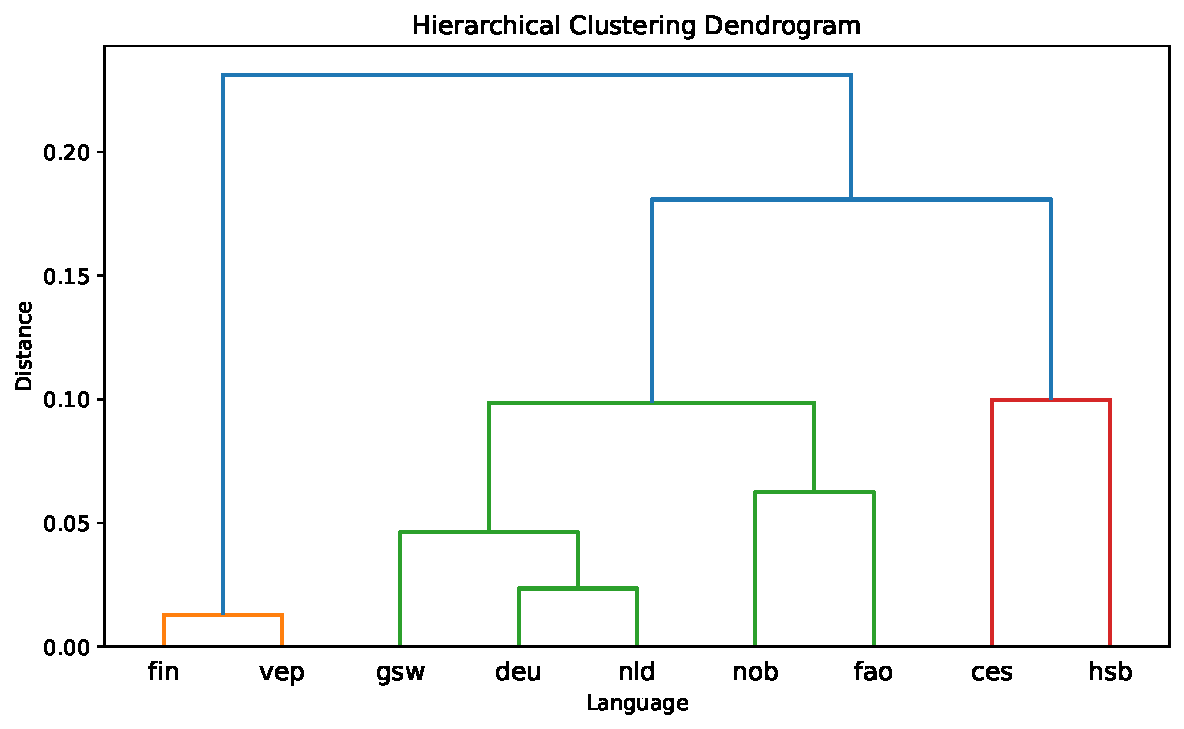
\includegraphics[width=0.75\linewidth]{figures/hcd.pdf}
			\caption{Agglomerative Hierarchical Clustering dendrogram based on the cosine similarity of the \texttt{syntax\_knn} vectors of the included languages.}
			\label{fig:hcd}
		\end{figure}

		The target languages are selected by finding the most typologically similar language to each of the auxiliary languages that have a UD treebank but  are not represented in M-BERT's pre-training data. For Dutch, the most similar language to meet the criteria is Swiss German, Norwegian is matched with Faroese, Czech with Upper Sorbian, and Finnish with Veps. The treebanks of the low-resource languages are randomly split into separate train, test, and validation sets as their treebanks do not contain these splits themselves.

	\subsection{Experiments}
	\label{sub:experiments}
		The research questions can be classified as evaluating the success of the setup or, more broadly, of typology-guided cross-lingual transfer (\textbf{Q1}, \textbf{Q2}, \textbf{Q3}) and as investigating how shifts in the model parameters facilitate cross-lingual transfer (\textbf{Q4}). Section~\ref{ssub:model_evaluation} outlines how the former group is answered, Section~\ref{ssub:probing_experiments} does the same for the latter.

		\subsubsection{Model Evaluation}
		\label{ssub:model_evaluation}
			Successful transfer is defined as higher performance on the target language test set. Following the example of Lauscher et al.~\cite{lauscher-etal-2020-zero}, the unlabeled attachment score (UAS) is used to quantify performance.\footnote{Using the more widely reported LAS would inhibit comparisons between datasets, as different treebanks may have been labeled with different annotation schemes.} In this section, the following notations are used:

			\begin{tabularx}{0.95\linewidth}{rrX}
				$l$ & & Any arbitrary language. \\
				$\ell$ & & Any arbitrary auxiliary language (Dutch, Norwegian, Czech, or Finnish). \\
				$\lambda$ & & Any arbitrary target language (Swiss German, Faroese, Upper Sorbian, or Veps). \\
				\m{l} & & A model finetuned on language $l$. If $l=\ell$, it is implied that it was first finetuned on German, as there are no cases where a model is directly finetuned on $\ell$ in this setup. \\
				\m{$l_1$,$l_2$} & & A language trained on $l_1$, then on $l_2$. \\
				\s{l_1}{l_2} & & Cosine similarity between the \texttt{syntax\_knn} vectors of $l_1$ and $l_2$. \\
				\uas{$l_1$}{l_2} & & The performance (in UAS) of \m{$l_1$} when evaluated on the test set of $l_2$. \\
				\dl{$l_3$}{$l_1$}{$l_2$} & & \uas{$l_1$}{l_3}$ - $\uas{$l_2$}{l_3}, i.e., the performance of \m{$l_2$} on $l_3$ subtracted from the performance of \m{$l_1$} on $l_3$. The value is positive when \m{$l_1$} performs better on $l_3$, negative when \m{$l_2$} performs better on $l_3$.
			\end{tabularx}

			\paragraph{Q1:} \textbf{Does greater typological similarity between the source and target languages result in better zero-shot cross-lingual transfer performance?}

				\noindent If typological similarity indeed leads to better zero-shot performance, the expectation is that \dl{$\lambda$}{$\ell$}{deu} is positive when \s{\ell}{\lambda} $>$ \s{\text{deu}}{\lambda}. That is, a model finetuned only on German would have worse zero-shot performance on $\lambda$ than a model that is finetuned on an $\ell$ that is typologically similar to $\lambda$. For example, \dl{fao}{nor}{deu} is expected to be positive because Norwegian is more typologically similar to Faroese than German is.

			\paragraph{Q2:} \textbf{To what degree does training on a few examples improve performance over zero-shot performance?}
			
				\noindent While Lauscher et al.~\cite{lauscher-etal-2020-zero} found training on as few as 10 examples to yield considerable improvements over zero-shot performance already, it is important to quantify the degree to which that holds in this setup. After Stage 3, the models \m{deu} and \m{$\ell$} are finetuned on 100 examples from $\lambda$. The result is twenty models \m{$l$,$\lambda$}. For each of those, improvement over zero-shot performance is defined as \dl{$\lambda$}{$l$,$\lambda$}{$l$}. Since training on a language is not expected to be detrimental to performance on that language, this value is not expected to ever be negative.

			\paragraph{Q3:} \textbf{Is training on a few examples from a target language more effective when first finetuning on a typologically similar auxiliary language?}

				\noindent This question can effectively be split into two components. Both are answered by investigating whether \dl{$\lambda$}{$l_1$,$\lambda$}{$l_2$,$\lambda$} is positive whenever \s{l_1}{\lambda} $>$ \s{l_2}{\lambda}. That is, performance on $\lambda$ is higher when the model finetuned to a language more similar to $\lambda$ in the preceding stage. One component of the question pertains to the effectiveness of the auxiliary stage in general. In this case, $l_1$ is any auxiliary language $\ell$ and $l_2$ is German. When $\ell$ is more similar to $\lambda$ than German is, the second stage may provide the model with new typological information that can then be leveraged in the third stage. The other component of the question pertains to the typological similarity between the auxiliary language and the target language. In this case, $l_1$ is any given auxiliary language and $l_2$ is any of the other auxiliary languages. This serves to assess whether any observed improvements are the result of typology, rather than longer training in general: if \m{ces,hsb} and \m{nld,hsb} score similarly on the Upper Sorbian test set, the impact of using an auxiliary language is separate from the typological similarity between the auxiliary and the target languages.

			% $\text{UAS}($\mbase$, L)$ is taken to be the UAS of \mbase evaluated on the test set of language $L$. Cosine similarity between URIEL's \texttt{syntax\_knn} vectors for languages $L1$ and $L2$ is denoted as $\text{s}(L1, L2)$. Moreover, as stated previously, $\ell$ is used for any of the auxiliary languages, $\lambda$ is used for any of the target languages. $\mathcal{L}$

		\subsubsection{Probing Experiments}
		\label{ssub:probing_experiments}
		Choenni \& Shutova~\cite{choenni-shutova-2022-investigating} used probing to investigate which features are encoded by a language model. That is, for each feature they investigate, they train a one-hidden-layer MLP that takes a sentence embedding of a sentence in a given language as input. The MLP is then tasked with predicting one of $n$ classes, with $n$ being the number of different ways a language can exhibit the feature at hand. If an MLP is able to classify a feature value based on a sentence embedding, the idea is then that the embedding encodes that feature.

		In this thesis, a similar approach is used, but instead training a probe to detect which language a sentence was written in based on its embedding. The embeddings are obtained from each of the 12 layers of the dependency parser's M-BERT-based encoder. Specifically, each token in a sentence is passed through the encoder to obtain token embeddings at each layer. A sentence embedding is then obtained by mean-pooling over the different token embeddings. This embedding is passed through a 100-dimensional hidden layer, followed by a softmax output layer that predicts which of the nine languages under scrutiny in this thesis a sentence was written in.

		Data for the probe is obtained from the Tatoeba corpora.\footnote{Available at \texttt{https://tatoeba.org}.\notetoself{Should be a hyperlink}} For each of the nine languages, 404 random sentences are sampled. This number was selected as Veps~-- the language with the smallest number of sentences available~-- has 404 sentences. Selecting this number of sentences for the other languages prevents issues caused by class imbalance. One half of these sentences is used in the training set, the other half is used in the test set. The probe is trained separately on each encoder and training spans 10 epochs with a learning rate of $1e\text{-}3$.

		\paragraph{Q4:} \textbf{Does finetuning on a language make its typological features more easily identifiable in the model's embedding space?}

		For this question, a language is heuristically taken to be a collection of its typological features. Identifiability of the features of language $l_1$ is then reflected by the probe's ability to correctly label sentences written in $l_1$, quantified as the F1-score.

		During finetuning on $l_1$, the model's encoder is tasked with generating an embedding that captures the typological features needed to construct an accurate dependency tree for $l_1$. Therefore, the features of $l_1$ are expected to be clearly represented in embeddings generated by the encoder of \m{$l_1$}. Since these features are generally distinct from those of typologically dissimilar languages, the probe is expected to perform worse on languages dissimilar to $l_1$. Conversely, the clearer encoding of the typological features of $l_1$ may lead to decreased separability of embeddings between $l_1$ and typologically similar languages. Consequently, the probe is expected to distinguish $l_1$ and typologically similar languages from languages that are more distant, but it will likely struggle to differentiate between $l_1$ and languages closely related to it.

		% \noindent For this question, identifiability of language $l_1$ is defined by how accurately a probe can detect whether a given sentence was written in language $l_1$ from the sentence's embedding. If finetuning on language $l_1$ makes its typological features more easily identifiable in the model's embedding space, it stands to reason that the accuracy of the probe in detecting $l_1$ consequently goes up. Moreover, a typologically similar $l_2$ has many of the same typological features. Therefore, if $l_1$ becomes more easily identifiable because its typological features are more clearly encoded, probe accuracy on detecting $l_2$ should go up as well.
